\section{Machine Learning Techniques}
\label{sec:ml-techniques}
\subsection{Traditional Machine Learning Techniques}
\label{subsec:concepts-traditional-techniques}
\begin{frame}{\insertsubsection}
    \begin{figure}
        \centering
        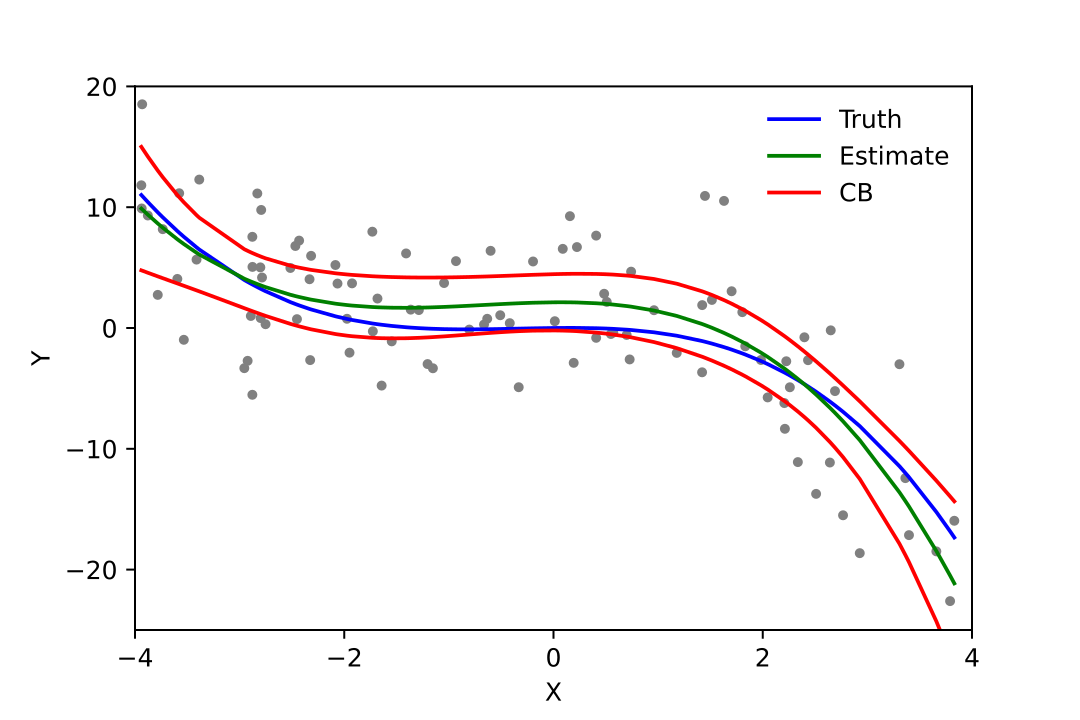
\includegraphics[width=0.8\textwidth]{media/Polyreg_scheffe.png}
        \caption{Polynomial Regression~\cite{Skbkekas2009}}
    \end{figure}
\end{frame}
%
%
\begin{frame}{\insertsubsection}
    \begin{figure}
        \centering
        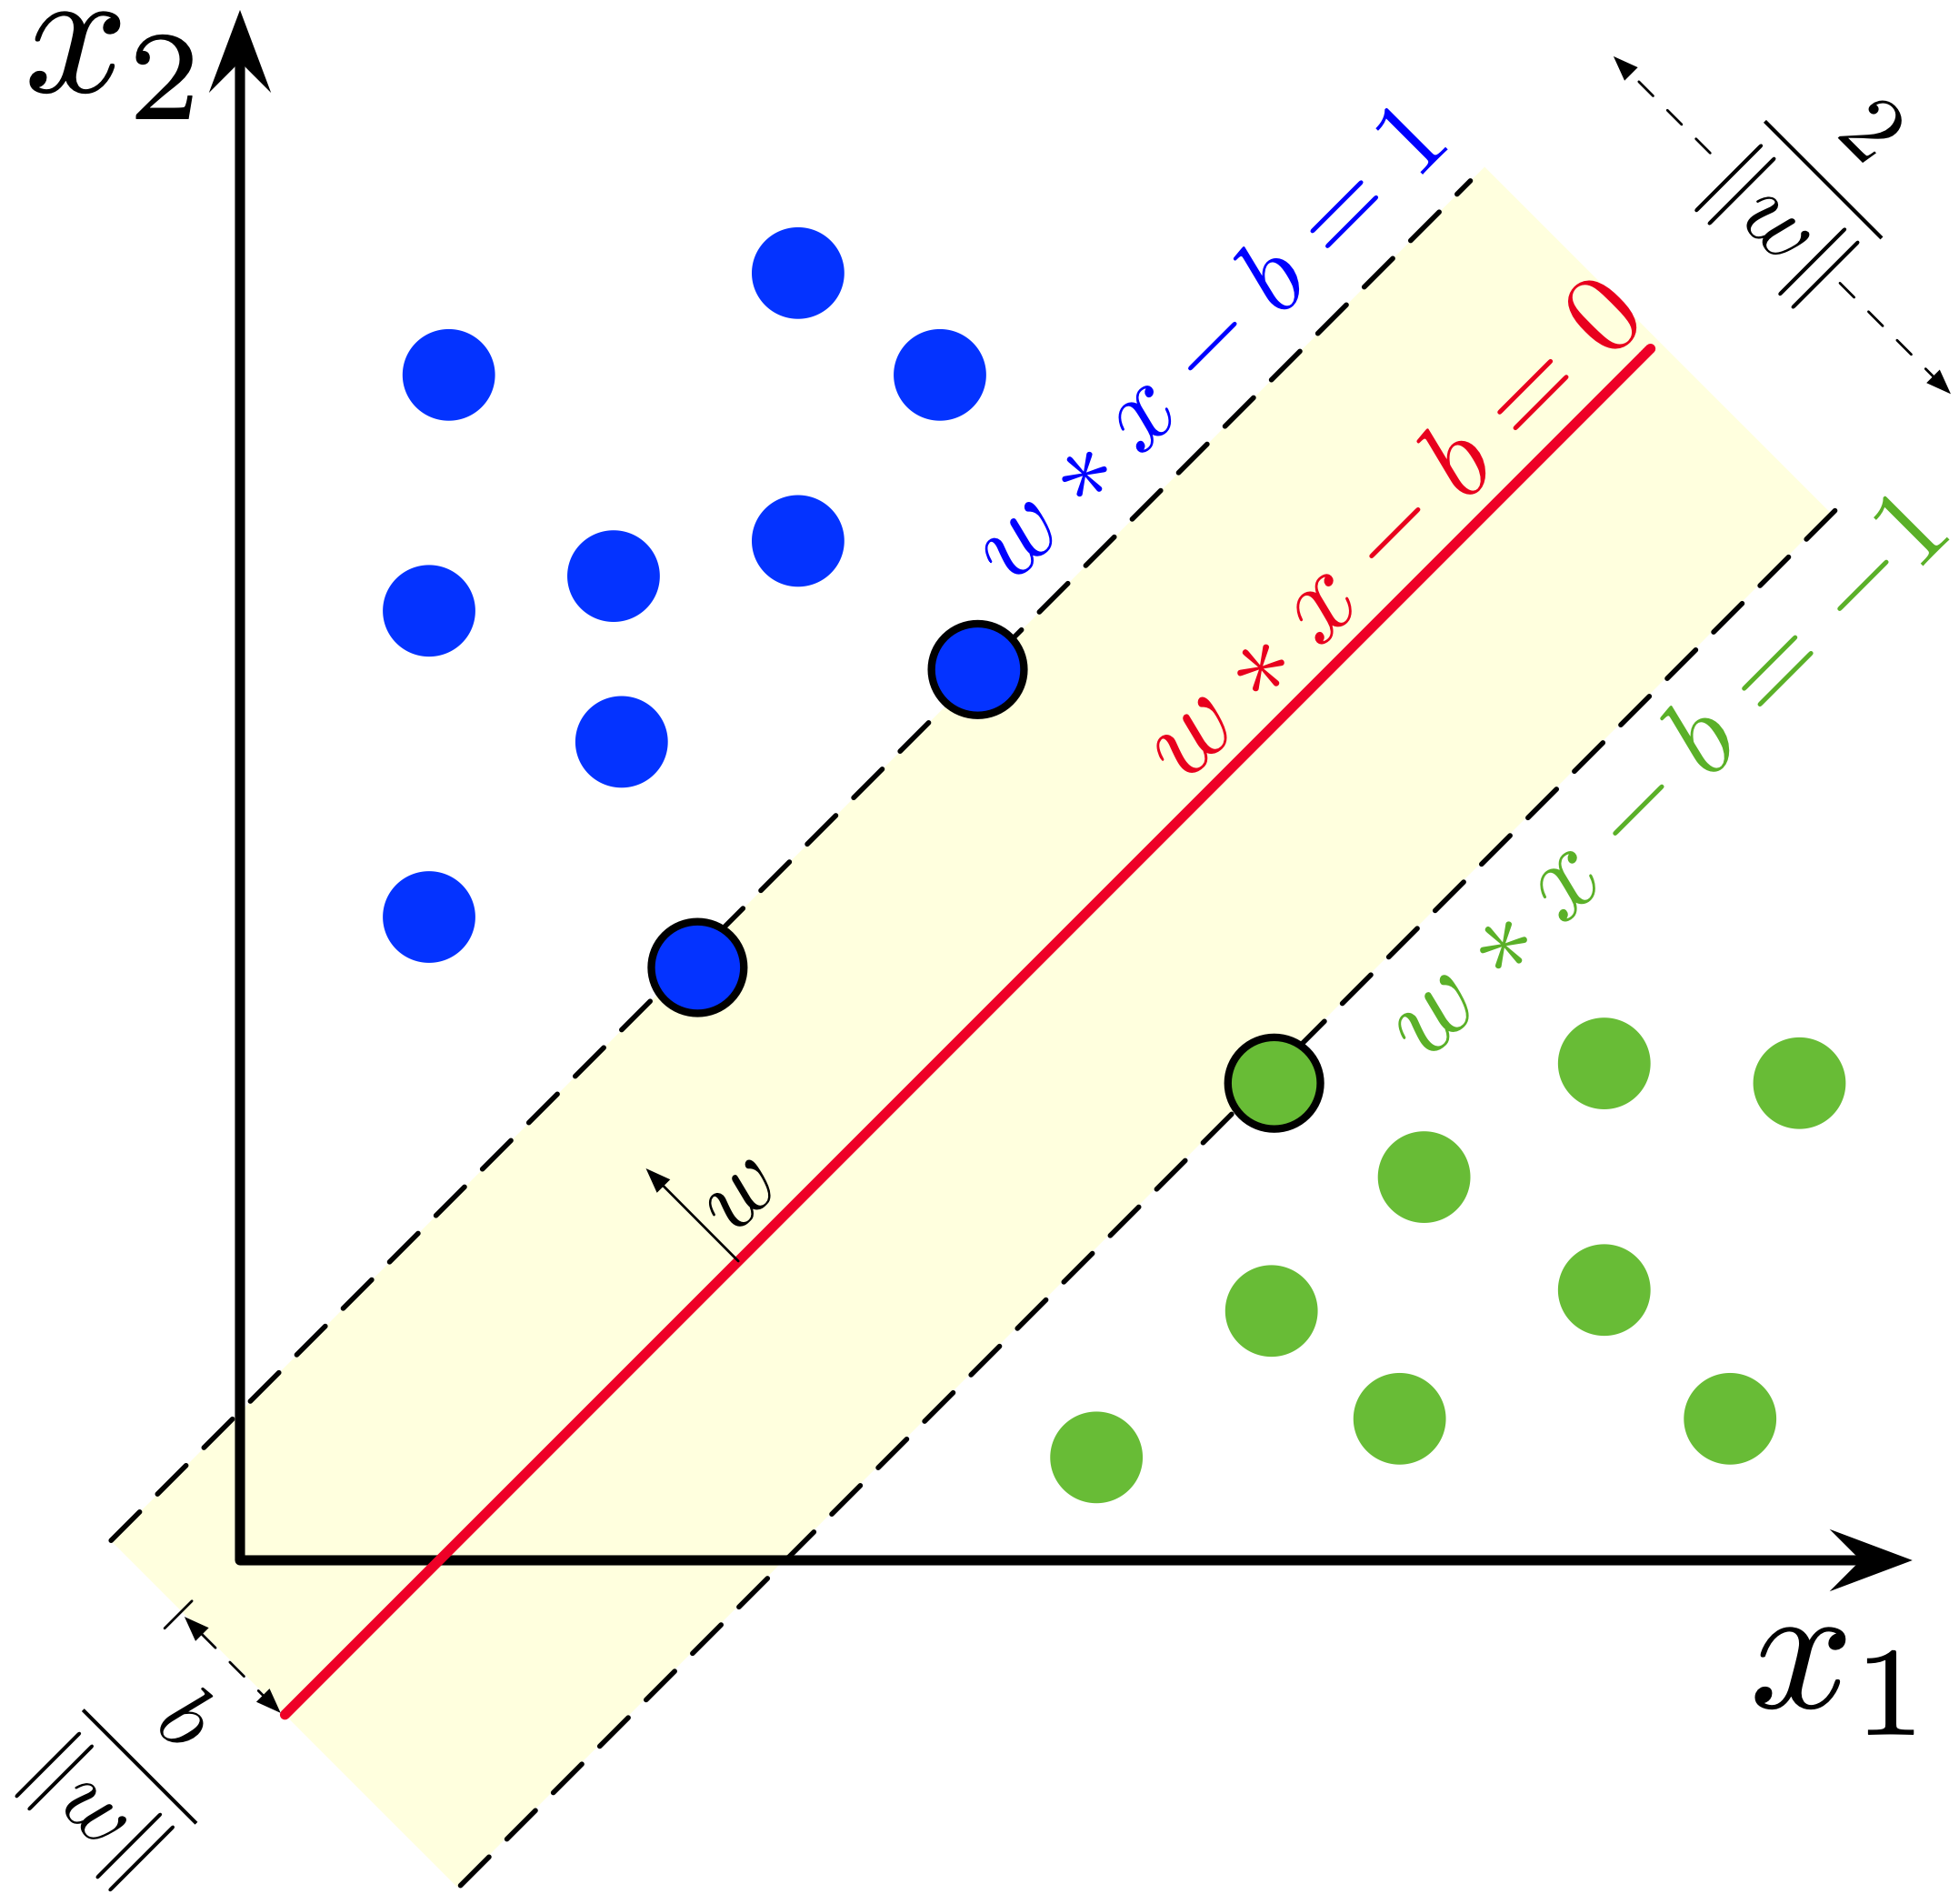
\includegraphics[width=0.6\textwidth]{media/SVM_margin.png}
        \caption{Support Vector Machine~\cite{Larhmam2018}}
    \end{figure}
\end{frame}
%
%
\begin{frame}{\insertsubsection}
    Traditional methods
    \begin{itemize}[<+->]
        \item Linear, polinomial, logistic regression
        \item Decision Trees
        \item[] Gradient boosting (eg. XGBoost)
        \item Support vector machine
        \item Random Forest
        \item Genetic Algorithms
    \end{itemize}
\end{frame}
%
%
\begin{frame}{\insertsubsection}
    \begin{itemize}
        \item Traditional machine learning routines should be preferred over neural networks
        \item Deep learning can be powerful (and trendy)
        \item[] However, currently still limited in applicability
        \item[] Requires lots of data $\Rightarrow$ often not present
        \item Traditional Methods are faster to develop and test
        \item[] They typically expect same number of features with each datapoint
        \item[] $\Rightarrow$ Padding and Windowing are methods to circumvent this
    \end{itemize}
\end{frame}
%
%
\subsection{Artificial Neural Networks}
\label{subsec:ml-techniques-deep-learning}
\begin{frame}{\insertsubsection}
    \begin{figure}
        \centering
        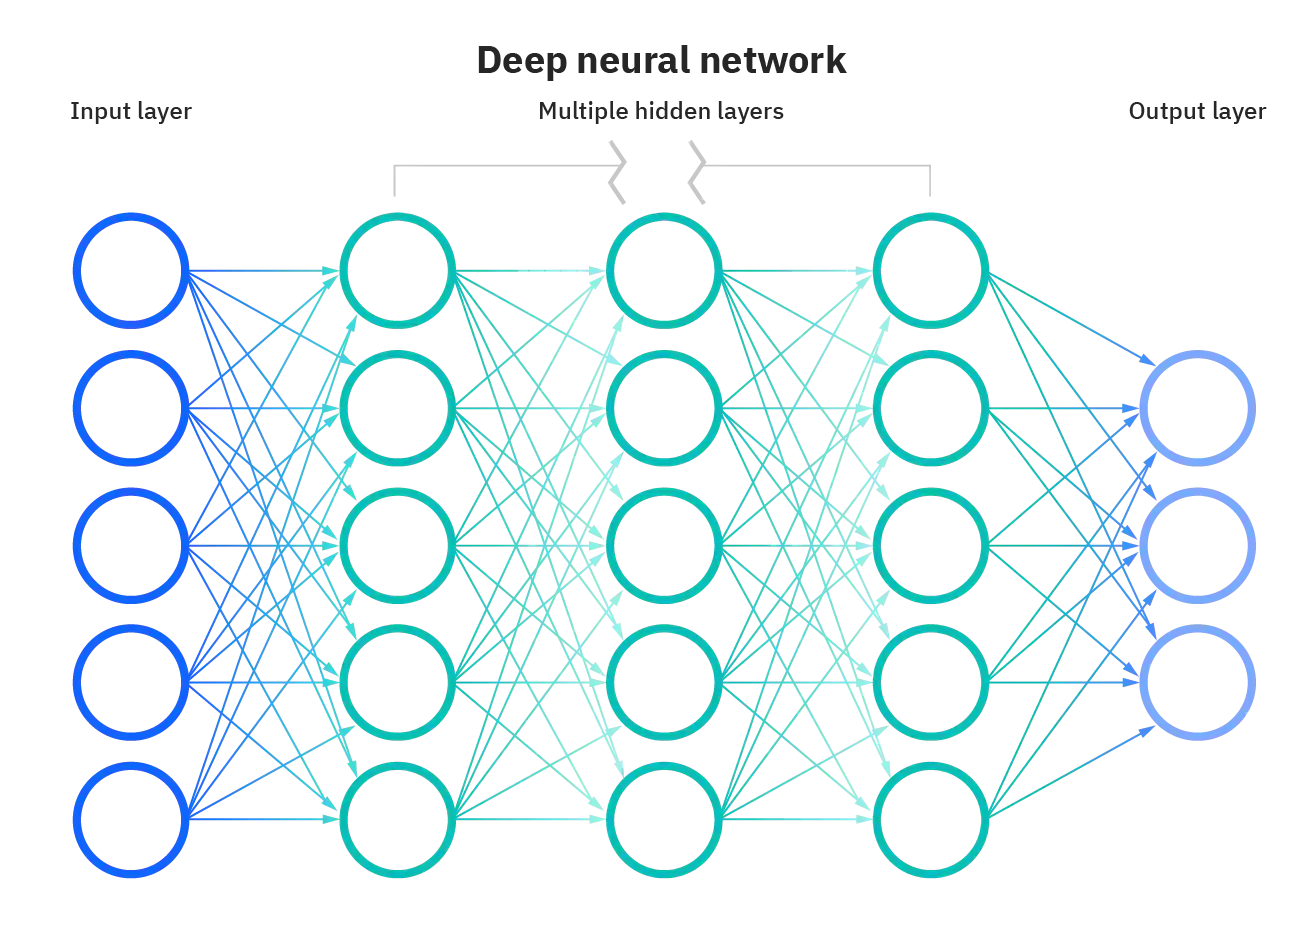
\includegraphics[width=0.8\textwidth]{media/ICLH_Diagram_Batch_01_03-DeepNeuralNetwork-WHITEBG.png}
        \caption{Standard, fully connected neural network~\cite{IBM2020}}
    \end{figure}
\end{frame}
%
%
\begin{frame}{\insertsubsection}
    \begin{itemize}
        \item Universal function approximators
        \item No guarantee that model will yield accurate predictins for new data
        \item Question: Is the trained model optimal?
        \item Neurons are at the heart of Neural Networks
        \item[] They apply a function to the input variables $x_i$ to obtain output $y$ by multiplying with learnable weight $w_i$.
        \begin{equation}
            y = \sigma\left(\sum\limits_{i=1}^n w_ix_i + b\right)
        \end{equation}
        \item Multiple layers $\Rightarrow$ iterate this procedure
    \end{itemize}
\end{frame}
%
%
\begin{frame}{\insertsubsection}
    \begin{figure}
        \centering
        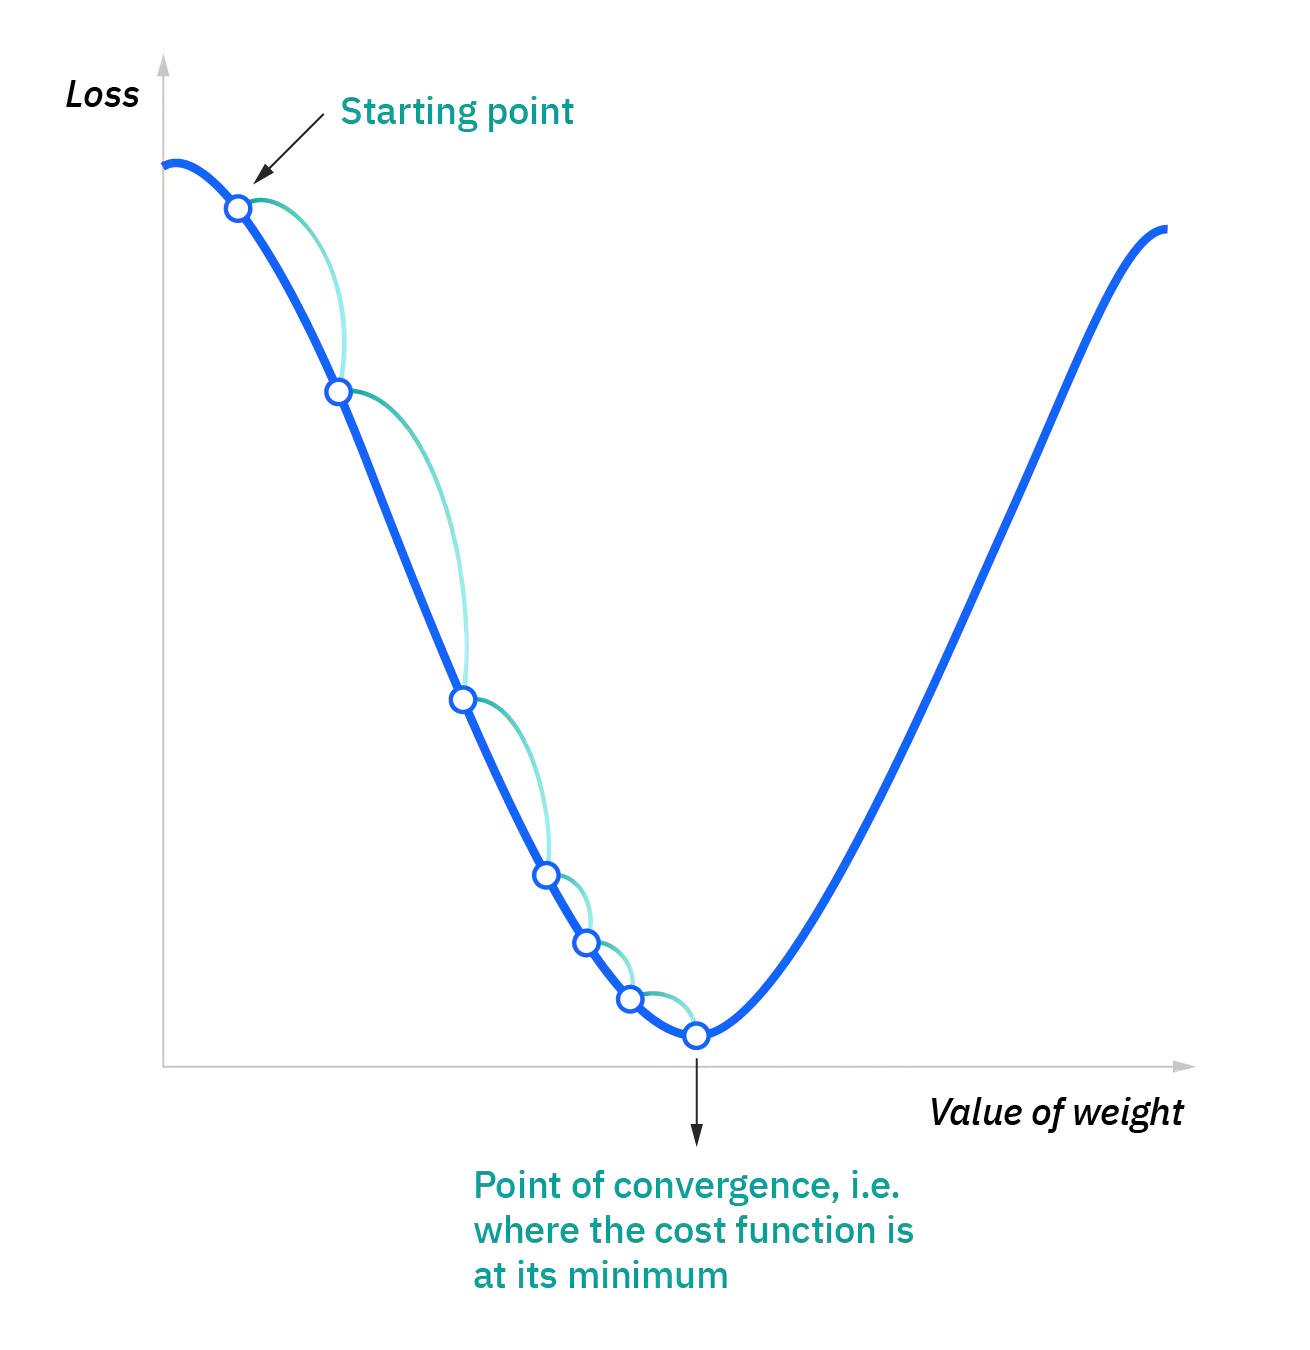
\includegraphics[width=0.35\textwidth]{media/ICLH_Diagram_Batch_01_04-GradientDescent-WHITEBG.png}
        \caption{Iterative approach to finding a local optimum of the cost function.
            It penalizes or rewards good/bad results. An example can be given by the mean squared error~\cite{IBM2020}.}
    \end{figure}
    \begin{equation}
        MSE = \frac{1}{2m}\sum\limits_{i=1}^m(\hat{y}-y)^2
    \end{equation}
\end{frame}
%
%
\subsection{Backpropagation}
\label{subsec:ml-techniques-backpropagation}
\begin{frame}{\insertsubsection}
    \begin{enumerate}[<+->]
        \item Let $g(x_i)$ be a network output of input variables $x_i$.
        \item Let $C(y_i, g(x_i))$ be the loss function for predicted output $g(x_i)$ and target output $y_i$.
        \item Let $W^l=(w^l_{jk})$ be the weights between layer $l-1$ and $l$ where $w^l_{jk}$ is the weight between $k$th node in layer $l-1$ and $j$th node in $l$.
        \item Calculate the gradient of loss function in weight-space for fixed input-output pair $(x_i,y_i)$
        \begin{equation}
            \frac{\partial C}{\partial w^l_{jk}}(y_i, g(x_i))
        \end{equation}
        \item Multiple layers in Neural Networks mean that $\partial C/\partial w$ needs to be evaluated by chain rule.
        \item[$\Rightarrow$] Modern Frameworks can do this process very efficiently.
        \item To optimize: Go along steepest negative gradient of $\partial C/\partial w$.
    \end{enumerate}
\end{frame}